\chapter{Implementation}
\label{4-practical}

\section{Functionality} 

PyWPS allows to publish and use geoprocessing services on a server. Every process that is to be implemented by PyWPS must be constructed as a Python class, contain a list of inputs nad outputs and a handler method with two parameters - request and response. Details on the procedure of creating new processes can be found in PyWPS documentation.\cite{pywpsprocess} 

To send a request to PyWPS, an instance of PyWPS must be running. If it is, the request is handled and a response is generated and returned to the client. The response has a form of an XML file and includes different elemenents depending on the type of the request.

When an Execute request is called, a new, temporary folder is created in location specified in configuration fil and input data is moved here. While the process is being executed, temporary files may be generated in this folder. For every process, it must be specified what the final output is. Once the execution is finished, the output is copied to a location that is accessible via the web. The temporary folder, containing input and output data and all the intermediate data that arose during the execution, is then deleted.

\subsection{Output Data Management}


\subsubsection{Current Options} 

The simplest option of delivering resulting data. When XML response is generated, output data is embedded in the document. Either as plain text, GML or, in case of an image, base64 scheme. This is typically used when the output is relatively small. It is also the default option.

\begin{figure}[H] \centering
      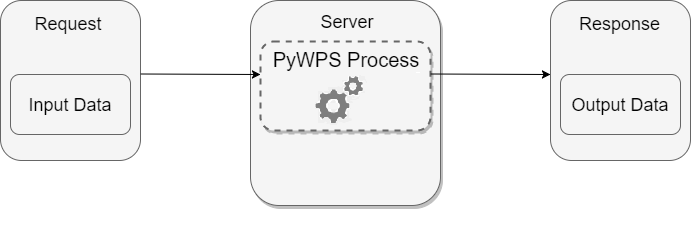
\includegraphics[width=350pt]{./pictures/optionone.png}
      \caption[Delivering data directly]{Delivering data directly}
      \label{fig:optionone}
  \end{figure}

If, on the contrary, the output data is large and complex, there is another option. The client is only given a reference, a URL link, from which the data can be downloaded. PyWPS saves the file in a folder specified in configuration passed by the service (or in a default location). The URL is embedded in the XML response.\cite{pywpsurl}

\begin{figure}[H] \centering
      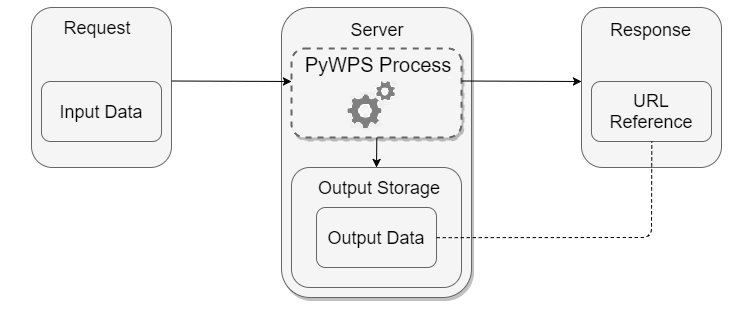
\includegraphics[width=370pt]{./pictures/optiontwo.png}
      \caption[Delivering data via URL reference]{Delivering data via URL reference}
      \label{fig:optiontwo}
  \end{figure}

It is up to the consumer of the process to decide which option to choose. For the latter option, the  "@asReference" value must be set to "True" in the request. By default, it is set to "False".


\subsubsection{Proposed Extension } 

The aim of this thesis was to develop another variant to add to the existing two that would store output data in a PostGIS database.

In such case, after the final output has been produced, connection to the database is established and the output data is copied there. When the XML response is delivered to the client, it contains a reference to the database with which the client can access the data. The reference is composed of the name of the database, schema and table. 

\begin{figure}[H] \centering
      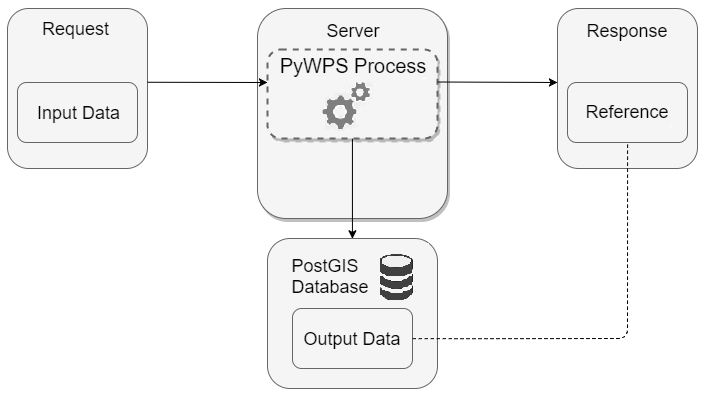
\includegraphics[width=350pt]{./pictures/newoption.png}
      \caption[Storing data in a database]{Storing data in a database}
      \label{fig:newoption}
  \end{figure}

The only difference from the previous two options when executing a process is that another input parameter must be included in the request. The parameter, db\textunderscore section, specifies the section from which the login credentials for connecting to the database are extracted in the configuration file.

To use this functionality as a consumer of a process, it must be implemented in the process by its author. For details on implementation when creating a process, please refer to the User Manual.


\section{Development} 

\subsection{PgStorage class development} 

A new class, PgStorage, has been developed that implements database storage support. It is a derived class, inheriting from StorageAbstract class that is a part of the standard PyWPS library. 

PgStorage is stored within the storage.py file in the .\textbackslash pywps\textbackslash inout folder. It consists of several methods that are described below. 

%co dal sem napsat?
\subsubsection{\textunderscore \textunderscore init\textunderscore \textunderscore } 
A constructor, i.e. it gets called automatically when an instance of the PgStorage class is created. 

In this method, the get\textunderscore config\textunderscore value function is used that is defined in the PyWPS API. It accesses the configuration file and retrieves required elements. What elements are retrieved is specified by the function's two parameters, section and option.

First, the name of the database is extracted from the configuration file and saved to a variable. Then, another variable is defined that serves as a connection string for connecting to a database. Requisite elements from the configuration file (user name, password and host server) are retrieved analogically. Finally, an instance of the create\textunderscore schema method is created and saved to a variable.

There are three parameters passed to the method - uuid, a unique string of every process, identifier (typically the name of the process) and the section name from the corresponding configuration file.

\subsubsection{create\textunderscore schema} 
First defines a variable schema\textunderscore name that consists of its two input parameters, separated by a dot - the identifier of the process and uuid.

Next, the psycopg2 library is used to connect to the database, specified by the "target" variable. A try-except clause is used to raise an exception if the connection could not be established. 

Then, when a cursor has been created, an SQL query is executed that generates a new schema if it doesn't exist already. Name of the schema is equal to the "schema\textunderscore name" variable. This, too, uses a try-except clause.

After the SQL query is performed, changes in the database are commited so they persist after connection is aborted, cursor and connection are closed and the schema\textunderscore name variable is returned.

\subsubsection{store\textunderscore output} 
As its name suggests, it handles writing output data to the database. It benefits from an extensive use of the OGR library. It has two input parameters, the name of the file that is to be stored in a database, and a process identifier. 

Thanks to OGR, the process is fairly simple and straight-forward. The output file is opened using the file name input parameter and connection to the database is established. Then, data is copied from the output file to the database using the OGR CopyLayer function. 

Each of the three above mentioned operations is followed by a simple condition that checks if the variable storing output of the operation is not None. If it is, it raises an exception with a corresponding message.


\subsubsection{store} 
Wraps the functionality of the store\textunderscore output method in a loop. If a process produces multiple output files, it applies the store\textunderscore output method's functionality for each file. 

Also, a string is created that specifies the location of the data. It consists of the name of the databse, schema and identifier of the process. This string is then given to the client as an output in the XML response of the process. The only input parameter of this method is the outputs of a process.


\subsection{Process class changes} 

The Process class is a part of the PyWPS source code. All processes inherit from this class. To use the (proposed functionality) there are a few changes that must be done in this code.

A new method must be defined that is called setOutputDbStorage. This can be done at the end of the current code. This method's only input parameter (in addition to the mandatory "self" parameter) is the name of the corresponding section in the configuration file. The method creates an instance of the PgStorage class and saves it in a variable.

Obviously, the name of the method is not restricted to the one stated above and it can be almost any string, however, this name must be used consistently throughout the process of setting up the extension.

Another snippet of code must be added at a specific location in one of the methods of the Process class, \textunderscore run\textunderscore process. It must be placed immediately after a response is created. The code is as follows:
\begin{verbatim}
            if hasattr(self, 'writer'):
                self.writer.store(self.outputs)
\end{verbatim}

It consists of a hasattr condition and a method call. The hasattr function is one of the functions built into the Python interpreter. It has two input parameters, a name of an object and a string. If the string is one of the object's attributes, it evaluates the condition as "True".\cite{hasattr} In this case, the object is "self" and the string is "writer". 

If the condition is met (i.e. the object - a process - does have an attribute called "writer") the second command is executed and the "store" method is called.

\subsection{Test} 

A script has been developed to test whether the process of storing outputs in a database functions correctly.

For the purpose of this test, three simple processes have been written. One of them only returns a string, other two (process\textunderscore one\textunderscore output and process\textunderscore two\textunderscore outputs) produce one and two complex outputs that are stored in a database. 

Both process\textunderscore one\textunderscore output and process\textunderscore two\textunderscore outputs generate buffers around input features, the latter also calculates centroids thereof. They are based on sample processes available for the PyWPS demo service. There is also a GML file provided with the demo service that was used as an input file for this test.  

To sucessfully run the test, instance of PyWPS must be running. When run, the test executes each of the processes and analyzis the corresponding XML response using the ElementTree XML parser. For every process, it returns an identifier of the process extracted from the XML document. 

For the two processes that yield complex outputs the test establishes connection to the database and counts features in the corresponding table. Then it compares this value to the number of features in the input file. If these two values differ, it raises an exception.

Similarly, it checks whether the geometry type of the layer in database is equal to a predefined value (point for centroids, polygon for buffer). If not, it raises an exception with a corresponding warning. 

When no exception is raised, it indicates that all processes have been run and all complex outputs have been stored in a database.

The OGR library is used for creating database connection, counting features and getting geometry type. Database login credentials are retrieved from a configuration file using get\textunderscore config\textunderscore value, a function built in the PyWPS library. To ensure correct configuration file is read, load\textunderscore configuration.





